\newcommand{\macro}[1]{{#1}} 

\newcommand\OoneSTART{\macro{September 12, 2015}}
\newcommand\OoneEND{\macro{January 19, 2016}}

\newcommand\OoneOfflineScienceHTimeSeconds{\macro{78.9~days}}
\newcommand\OoneOfflineScienceLTimeSeconds{\macro{67.2~days}}
\newcommand\OoneOfflineScienceTimeSeconds{\macro{51.3~days}}

\newcommand\OoneOfflineAnalysableHTimeSeconds{\macro{76.7~days}}
\newcommand\OoneOfflineAnalysableLTimeSeconds{\macro{65.8~days}}
\newcommand\OoneOfflineAnalysableTimeYears{\macro{0.13~years}}
\newcommand\OoneOfflineAnalysableTimeSeconds{\macro{49.0~days}}

\newcommand\OoneOfflineAnalysableCatTwoHTimeSeconds{\macro{75.9~days}}
\newcommand\OoneOfflineAnalysableCatTwoLTimeSeconds{\macro{65.8~days}}
\newcommand\OoneOfflineAnalysableCatTwoTimeSeconds{\macro{48.5~days}}
\newcommand\OoneOfflineAnalysableCatTwoDiffSeconds{\macro{0.5~days}}

\newcommand\OoneOfflineAnalysedBOTHTimeDays{\macro{48~days}}

\newcommand\OoneOnlineAnalysableTimeSeconds{\macro{52.2~days}}

\newcommand\OoneOnlineAnalysableTimeNotAnalysableOfflineSeconds{\macro{3.2~days}}

\newcommand\OoneOnlineAnalysedMBTATimeSeconds{\macro{50.5~days}}
\newcommand\OoneOnlineAnalysedMBTATimePercent{\macro{96.6~\%}}

\newcommand\OoneOnlineAnalysedGSTLALTimeSeconds{\macro{49.4~days}}

\newcommand\OoneOnlineAnalysedGSTLALTimePercent{\macro{94.6~\%}}
\newcommand\OoneOnlineAnalysedBOTHTimeSeconds{\macro{52.0~days}}
\newcommand\OoneOnlineAnalysedBOTHTimePercent{\macro{99.5~\%}}


\newcommand\OoneOnlineTotalMBTAGraceDBEvents{\macro{486}}
\newcommand\OoneOnlineTotalGSTLALGraceDBEvents{\macro{868}}
\newcommand\OoneOnlineTotalEMFollowUpEvents{\macro{8}}


\newcommand\LVBLAHsignificance{\macro{$1.7 \sigma$}}

\newcommand\MainBNSULLowSpin{\macro{\MainBNSULPyCBCLowSpin}}
\newcommand\MainBNSULHighSpin{\macro{\MainBNSULPyCBCHighSpin}}
\newcommand\MainBNSULPyCBCLowSpin{\macro{12,100}}
\newcommand\MainBNSULPyCBCHighSpin{\macro{12,600}}
\newcommand\MainBNSULGstlalLowSpin{\macro{11,500}}
\newcommand\MainBNSULGstlalHighSpin{\macro{12,200}}

\newcommand\SSixULNoSpin{\macro{130,000 $\mathrm{Gpc}^{-3}$ $\mathrm{yr}^{-1}$}}

\newcommand\MainBNSVTLowSpin{\macro{\MainBNSVTPyCBCLowSpin}}
\newcommand\MainBNSVTHighSpin{\macro{\MainBNSVTPyCBCHighSpin}}
\newcommand\MainBNSVTPyCBCLowSpin{\macro{$2.09\times 10^{-4}$}}
\newcommand\MainBNSVTPyCBCHighSpin{\macro{$2.00\times 10^{-4}$}}
\newcommand\MainBNSVTGstlalLowSpin{\macro{$2.20\times 10^{-4}$}}
\newcommand\MainBNSVTGstlalHighSpin{\macro{$2.07\times 10^{-4}$}}

\newcommand\MainBNSRangePyCBCLowSpin{\macro{73.2}}
\newcommand\MainBNSRangePyCBCHighSpin{\macro{72.1}}
\newcommand\MainBNSRangeGstlalLowSpin{\macro{73.4}}
\newcommand\MainBNSRangeGstlalHighSpin{\macro{72.0}}

\newcommand\MainNSBHULFiveIso{\macro{\MainNSBHULPyCBCFiveIso}}
\newcommand\MainNSBHULTenIso{\macro{\MainNSBHULPyCBCTenIso}}
\newcommand\MainNSBHULThirtyIso{\macro{\MainNSBHULPyCBCThirtyIso}}
\newcommand\MainNSBHULFiveAligned{\macro{\MainNSBHULPyCBCFiveAligned}}
\newcommand\MainNSBHULTenAligned{\macro{\MainNSBHULPyCBCTenAligned}}
\newcommand\MainNSBHULThirtyAligned{\macro{\MainNSBHULPyCBCThirtyAligned}}
\newcommand\MainNSBHVTFiveIso{\macro{\MainNSBHVTPyCBCFiveIso}}
\newcommand\MainNSBHVTTenIso{\macro{\MainNSBHVTPyCBCTenIso}}
\newcommand\MainNSBHVTThirtyIso{\macro{\MainNSBHVTPyCBCThirtyIso}}
\newcommand\MainNSBHVTFiveAligned{\macro{\MainNSBHVTPyCBCFiveAligned}}
\newcommand\MainNSBHVTTenAligned{\macro{\MainNSBHVTPyCBCTenAligned}}
\newcommand\MainNSBHVTThirtyAligned{\macro{\MainNSBHVTPyCBCThirtyAligned}}

\newcommand\MainNSBHULPyCBCFiveIso{\macro{3,600}}
\newcommand\MainNSBHULPyCBCTenIso{\macro{2,530}}
\newcommand\MainNSBHULPyCBCThirtyIso{\macro{2,300}}
\newcommand\MainNSBHULPyCBCFiveAligned{\macro{3,210}}
\newcommand\MainNSBHULPyCBCTenAligned{\macro{1,850}}
\newcommand\MainNSBHULPyCBCThirtyAligned{\macro{1,280}}
\newcommand\MainNSBHVTPyCBCFiveIso{\macro{$7.01\times 10^{-4}$}}
\newcommand\MainNSBHVTPyCBCTenIso{\macro{$1.00\times 10^{-3}$}}
\newcommand\MainNSBHVTPyCBCThirtyIso{\macro{$1.10\times 10^{-3}$}}
\newcommand\MainNSBHVTPyCBCFiveAligned{\macro{$7.87\times 10^{-4}$}}
\newcommand\MainNSBHVTPyCBCTenAligned{\macro{$1.36\times 10^{-3}$}}
\newcommand\MainNSBHVTPyCBCThirtyAligned{\macro{$1.98\times 10^{-3}$}}
\newcommand\MainNSBHRangePyCBCFiveIso{\macro{110}}
\newcommand\MainNSBHRangePyCBCTenIso{\macro{123}}
\newcommand\MainNSBHRangePyCBCThirtyIso{\macro{127}}
\newcommand\MainNSBHRangePyCBCFiveAligned{\macro{114}}
\newcommand\MainNSBHRangePyCBCTenAligned{\macro{137}}
\newcommand\MainNSBHRangePyCBCThirtyAligned{\macro{155}}

\newcommand\MainNSBHULGstlalFiveIso{\macro{3,270}}
\newcommand\MainNSBHULGstlalTenIso{\macro{2,490}}
\newcommand\MainNSBHULGstlalThirtyIso{\macro{2,800}}
\newcommand\MainNSBHULGstlalFiveAligned{\macro{2,820}}
\newcommand\MainNSBHULGstlalTenAligned{\macro{1,660}}
\newcommand\MainNSBHULGstlalThirtyAligned{\macro{1,270}}
\newcommand\MainNSBHVTGstlalFiveIso{\macro{$7.71\times 10^{-4}$}}
\newcommand\MainNSBHVTGstlalTenIso{\macro{$1.01\times 10^{-3}$}}
\newcommand\MainNSBHVTGstlalThirtyIso{\macro{$9.02\times 10^{-4}$}}
\newcommand\MainNSBHVTGstlalFiveAligned{\macro{$8.96\times 10^{-4}$}}
\newcommand\MainNSBHVTGstlalTenAligned{\macro{$1.52\times 10^{-3}$}}
\newcommand\MainNSBHVTGstlalThirtyAligned{\macro{$1.99\times 10^{-3}$}}
\newcommand\MainNSBHRangeGstlalFiveIso{\macro{112}}
\newcommand\MainNSBHRangeGstlalTenIso{\macro{122}}
\newcommand\MainNSBHRangeGstlalThirtyIso{\macro{118}}
\newcommand\MainNSBHRangeGstlalFiveAligned{\macro{117}}
\newcommand\MainNSBHRangeGstlalTenAligned{\macro{140}}
\newcommand\MainNSBHRangeGstlalThirtyAligned{\macro{153}}


\newcommand\SSixNSBHULFiveNoSpin{\macro{31,000 $\mathrm{Gpc}^{-3}$ $\mathrm{yr}^{-1}$}}
\newcommand\SSixNSBHULFiveSpin{\macro{36,000 $\mathrm{Gpc}^{-3}$ $\mathrm{yr}^{-1}$}}

\newcommand\MainBNSRange{\macro{$\sim$ 70 $\mathrm{Mpc}$}}
\newcommand\MainNSBHRangeFive{\macro{$\sim$ 110 $\mathrm{Mpc}$}}
\newcommand\MainNSBHRangeTen{\macro{$\sim$ 120 $\mathrm{Mpc}$}}

\newcommand\GRBBNSBeamingAngleConstraint{\macro{${2.3^{+1.7}_{-1.1}}^{\circ}$}}
\newcommand\GRBNSBHFiveBeamingAngleConstraint{\macro{${4.3^{+3.1}_{-1.9}}^{\circ}$}}
\newcommand\GRBNSBHTenBeamingAngleConstraint{\macro{${5.1^{+3.7}_{-2.3}}^{\circ}$}}
\newcommand\GRBNSBHThirtyBeamingAngleConstraint{\macro{${5.3^{+3.9}_{-2.4}}^{\circ}$}}



\acrodef{aLIGO}[aLIGO]{Advanced Laser Interferometer Gravitational Wave Observatory}
\acrodef{BBH}[BBH]{binary black-hole}
\acrodef{BH}[BH]{black-hole}
\acrodef{BNS}[BNS]{binary neutron-star}
\acrodef{CBC}[CBC]{compact binary coalescence}
\acrodef{EM}[EM]{electromagnetic}
\acrodef{GraCEDb}[GraCEDb]{gravitational-wave candidate event database}
\acrodef{GRB}[GRB]{gamma-ray burst}
\acrodef{GW}[GW]{gravitational wave}
\acrodef{LIGO}[LIGO]{Laser Interferometer Gravitational Wave Observatory}
\acrodef{NS}[NS]{neutron-star}
\acrodef{NSBH}{neutron-star--black-hole}
\acrodef{O1}[O1]{first observing period}

\section{Introduction}
The content of this chapter are primarily taken from ``Upper Limits on the Rates of Binary Neutron Star and Neutron-Star–Black-Hole Mergers from Advanced LIGO’S First Observing Run" in 2016. The main focus is on the results from the PyCBC offline search analysis conducted in this study.

Between \OoneSTART\ and \OoneEND\, the two advanced \ac{LIGO} detectors conducted their \ac{O1}.
During \ac{O1}, two high-mass \ac{BBH} events
were identified with high confidence ($> 5 \sigma$): GW150914~\citep{Abbott:2016blz} and
GW151226~\citep{Abbott:2016nmj}. A third signal, LVT151012, was
also identified with \LVBLAHsignificance\ confidence~\citep{TheLIGOScientific:2016pea, TheLIGOScientific:2016qqj}
In all three cases the component masses are confidently constrained to be above the $3.2M_\odot$ upper mass limit of \acp{NS} set
by theoretical considerations~\citep{Rhoades:1974fn,TheLIGOScientific:2016wfe}.
The details of these observations, investigations about the properties
of the observed \ac{BBH} mergers, and the astrophysical implications are explored
in~\citep{TheLIGOScientific:2016wfe,Abbott:2016nhf,TheLIGOScientific:2016htt,TheLIGOScientific:2016src,TheLIGOScientific:2016pea, Abbott:2016izl}.

The search methods that successfully observed these \ac{BBH} mergers also target other types of compact
binary coalescences, specifically the inspiral and merger of \ac{BNS} systems and \ac{NSBH} systems. Such systems were considered
among the most promising candidates for an observation in \ac{O1}. For example, a simple calculation
prior to the start of O1 predicted 0.0005 - 4 detections of \ac{BNS}
signals during O1~\citep{Aasi:2013wya}.

n this paper we report on the search for \ac{BNS} and \ac{NSBH} mergers in \ac{O1}. We have
searched for \ac{BNS} systems with component masses $\in [1,3] M_{\odot}$, component dimensionless
spins $< 0.05$ and spin orientations aligned or anti-aligned with the orbital angular momentum.
We have searched for \ac{NSBH} systems with neutron star mass $\in [1,3] M_{\odot}$,
\ac{BH} mass $\in [2,99] M_{\odot}$ neutron star dimensionless spin magnitude $< 0.05$,
\ac{BH} dimensionless spin magnitude $<0.99$ and both spins
aligned or anti-aligned with the orbital angular momentum.
No observation of
either \ac{BNS} or \ac{NSBH} mergers was made in \ac{O1}. We explore the astrophysical implications
of this result, placing upper limits on the rates of such merger events in the
local Universe that
are roughly an order of magnitude smaller than those obtained with data from Initial \ac{LIGO}
and Initial Virgo~\citep{Abbott:2007kv,Acernese:2008zzf,Colaboration:2011np}.
We compare these updated rate limits to current predictions of \ac{BNS} and
\ac{NSBH} merger rates and explore how the non-detection of \ac{BNS} and \ac{NSBH} systems in \ac{O1} can be used
to explore possible constraints of the opening angle of the radiation cone of short \acp{GRB},
assuming that short \ac{GRB} progenitors are \ac{BNS} or \ac{NSBH} mergers.

The layout of this paper is as follows. In \S\,~\ref{sec:source_considerations} we describe
the motivation for our search parameter space. In \S\,~\ref{sec:search_description} we briefly
describe the search methodology, then describe the results of the search in \S\,~\ref{sec:search_results}.
We then discuss the constraints that can be placed on the rates of \ac{BNS} and \ac{NSBH} mergers in \S\,~\ref{sec:rates}
and the astrophysical implications of the rates in \S\,~\ref{sec:astrophys_interp}. Finally, we conclude
in \S\,~\ref{sec:conclusion}.

\section{Source considerations}
\label{sec:source_considerations}

There are currently thousands of known NSs, most detected as pulsars
\citep{pulsarcat,Manchester:2004bp}. Of these, $\sim70$ are found in binary
systems and allow estimates of the NS mass
\citep{nsmassespage,Lattimer:2012nd,Ozel:2016oaf}.
Published mass estimates range from $1.0\pm0.17\,{M_{\odot}}$ \citep{Falanga:2015mra} to
$2.74\pm0.21\,{{M_{\odot}}}$ \citep{Freire:2007jd} although there is some uncertainty
in some of these measurements.
Considering only precise mass measurements from these observations one can set a lower bound
on the maximum possible neutron star mass of $2.01\pm 0.04\,{M_{\odot}}$~\citep{Antoniadis:2013pzd} and theoretical considerations
set an upper bound on the maximum possible neutron star mass of $2.9$--$3.2\,{M_{\odot}}$ \citep{Rhoades:1974fn,Kalogera:1996ci}.
The standard formation scenario of core-collapse supernovae restricts the birth
masses of neutron stars to be above $1.1$--$1.6\,{M_{\odot}}$
\citep{Ozel:2012ax,Lattimer:2012nd,Kiziltan:2013oja}.

Eight candidate \ac{BNS} systems allow mass measurements for individual
components, giving a much narrower mass distribution~\citep{Lorimer:2008se}. Masses are
reported between $1.0\,{{M_{\odot}}}$ and
$1.49\,{{M_{\odot}}}$~\citep{nsmassespage,Ozel:2016oaf}, and are consistent with an
underlying mass distribution of $(1.35 \pm
0.13)\,{{M_{\odot}}}$~\citep{Kiziltan:2010ct}.
These observational measurements assume masses are greater than $0.9{{M_{\odot}}}$.

The fastest spinning pulsar observed so far rotates with a frequency of 716\,Hz~\citep{Hessels:2006ze}. This
corresponds to a dimensionless spin $\chi = c | \mathbf{S} | / G m^2$ of roughly 0.4, where $m$ is the object's
mass and  $\mathbf{S}$ is the angular momentum.\footnote{Assuming a mass of $1.4{{M_\odot}}$ and
a moment of inertia $=J/\Omega$ of $1.5\times10^{45}$\,g\,cm$^2$; the exact moment of
inertia is dependent on the unknown \ac{NS} equation-of-state~\citep{Lattimer:2012nd}.} Such
rapid rotation rates likely require the NS to have been spun up through mass-transfer
from its companion. The fastest spinning pulsar in a confirmed \ac{BNS} system has a
spin frequency of 44\,Hz~\citep{Kramer:2009zza}, implying that dimensionless
spins for NS in \ac{BNS} systems are $\leq 0.04$~\citep{Brown:2012qf}. However,
recycled NS can have larger spins, and the potential \ac{BNS} pulsar J1807-2500B
\citep{Lynch:2011aa} has
a spin of 4.19\,ms, giving a dimensionless spin of up to
$\sim0.2$.\footnote{Calculated with a pulsar mass of $1.37{{M_\odot}}$ and a
high moment of inertia, $2\times10^{45}$\,g\,cm$^2$.}

Given these considerations, we search for \ac{BNS} systems with both masses
$\in [1,3] M_{\odot}$ and component dimensionless spins $< 0.05$. We have found
that \ac{BNS} systems with spins $< 0.4$ are generally still recovered well even
though they are not explicitly covered by our search space. Increasing the
search space to include \ac{BNS} systems with spins $< 0.4$ was found to
not improve overall search sensitivity~\citep{nitzthesis}.

\ac{NSBH} systems are thought to be efficiently formed in one of two ways: either
through the stellar evolution of field binaries or through dynamical
capture of a \ac{NS} by a \ac{BH}~\citep{Grindlay:2005ym,Sadowski:2007dz,Lee:2009ca,Benacquista:2011kv}.
Though no \ac{NSBH} systems are known to
exist, one likely progenitor has been observed, Cyg
X-3~\citep{Belczynski:2012jc}.

Measurements of galactic stellar mass
\acp{BH} in X-ray binaries yield \ac{BH} masses
$5 \le M_{\rm BH}/{M_{\odot}}\le 24$~\citep{Farr:2010tu,Ozel:2010su,Merloni:2008tj,Wiktorowicz:2013dua}.
Extragalactic high-mass X-ray binaries, such as IC10 X-1 and NGC300 X-1 suggest
BH masses of $20-30\,{M_{\odot}}$. Advanced \ac{LIGO} has observed two definitive \ac{BBH} systems and
constrained the masses of the 4 component \acp{BH} to $36_{-4}^{+5},
29_{-4}^{+4}, 14_{-4}^{+8}$ and $7.5_{-2.3}^{+2.3}\,M_{\odot}$, respectively, and
the masses of the two resulting \acp{BH} to $62_{-4}^{+4}$ and
$21_{-2}^{+6}\,M_{\odot}$. In addition if one assumes that the candidate \ac{BBH} merger LVT151012
was of astrophysical origin than its component \acp{BH} had masses constrained to $23_{-6}^{+16}$
and $13_{-5}^{+4}$ with a resulting \ac{BH} mass of $35_{-4}^{+14}$.
There is an apparent gap of \acp{BH} in the mass range $3$--$5\,
{M_{\odot}}$, which has been ascribed to the supernova explosion
mechanism~\citep{Belczynski:2011bn,Fryer:2011cx}. However, \acp{BH} formed from stellar
evolution may exist with masses down to $2\,{M_{\odot}}$, especially if they are formed
from matter accreted onto neutron stars \citep{O'Shaughnessy:2005qc}.
Population synthesis models typically allow for stellar-mass \ac{BH} up to
$\sim 80\text{--}100\,{M_{\odot}}$~\citep{Fryer:2011cx,Belczynski:2009xy,Dominik:2012kk};
stellar \acp{BH} with mass above $100\,{M_{\odot}}$ are also conceivable however
\citep{Belczynski:2014iua,deMink:2015yea}.

X-ray observations of accreting \acp{BH} indicate a broad
distribution of \ac{BH} spin~\citep{Miller:2009cw,Shafee:2005ef,
McClintock:2006xd,Liu:2008tk,Gou:2009ks,Davis:2006cm, Li:2004aq,Miller:2014aaa}.
Some \acp{BH} observed in X-ray binaries have very large dimensionless spins
(e.g Cygnus X-1 at $>0.95$ \citep{2012MNRAS.424..217F,Gou:2011nq}), while others
could have much lower spins ($\sim 0.1$)~\citep{McClintock:2011zq}. Measured
\ac{BH} spins in high-mass X-ray binary systems tend to have large values ($>0.85$), and
these systems are more likely to be progenitors of \ac{NSBH}
binaries~\citep{McClintock:2013vwa}.  Isolated \ac{BH} spins are only constrained
by the relativistic Kerr bound ${\chi} \leq 1$~\cite{misner2017gravitation}.
LIGO's observations of merging binary \ac{BH} systems yield
weak constraints on component spins \citep{TheLIGOScientific:2016wfe,Abbott:2016nmj,TheLIGOScientific:2016pea}.
The microquasar XTE J1550-564~\citep{Steiner:2011vr} and population synthesis
models~\citep{Fragos:2010tm} indicate small spin-orbit misalignment in
field binaries.
Dynamically formed \ac{NSBH} systems, in contrast, are expected to
have no correlation between the spins and the orbit.

We search for \ac{NSBH} systems with NS mass
$\in [1,3] M_{\odot}$, NS dimensionless spins $< 0.05$, BH mass $\in [2,99] M_{\odot}$
and BH spin magnitude $< 0.99$. Current search techniques are restricted to
waveform models where the spins are (anti-)aligned with the orbit~\citep{Messick:2016aqy,Usman:2015kfa},
although methods to extend this to generic spins are being explored~\citep{Harry:2016ijz}.
Nevertheless, aligned-spin searches have been shown to have good sensitivity
to systems with generic spin orientations in \ac{O1}~\citep{dal2015impact,Harry:2016ijz}. An
additional search for BBH systems with total mass greater than 100 $M_{\odot}$
is also being performed, the results of which will be reported in a future publication.

\section{Search Description}
\label{sec:search_description}

To observe compact binary coalescences in data taken from Advanced \ac{LIGO} we use
matched-filtering against models of compact binary merger \ac{GW} signals~\citep{Wainstein}.
Matched-filtering has long been the primary tool for modeled \ac{GW} searches~\citep{Abbott:2003pj, Colaboration:2011np}.
As the emitted \ac{GW} signal varies significantly over the range of masses and spins
in the \ac{BNS} and \ac{NSBH} parameter space, the matched-filtering process must be repeated
over a large set of filter waveforms, or ``template bank''~\citep{Owen:1998dk}.
The ranges of masses considered in the searches are shown in Figure~\ref{fig:banks}.
The matched-filter process is conducted independently for each of the two \ac{LIGO} observatories before searching
for any potential \ac{GW} signals observed at both observatories with the
same masses and spins and within the expected light travel time delay.
A summary statistic is then assigned to each coincident event based on the estimated
rate of false alarms produced by the search background that would be more significant than the event.

\ac{BNS} and \ac{NSBH} mergers are prime candidates not only for observation with
\ac{GW} facilities, but also for coincident observation with \ac{EM}
observatories~\citep{Eichler:1989ve, Hansen:2000am, Narayan:1992iy, Li:1998bw, Nakar:2007yr, Metzger:2011bv, Nakar:2011cw, Berger:2013jza, Zhang:2013lta, Fong:2015oha}.
We have a long history of working with the Fermi, Swift and IPN \ac{GRB} teams
to perform sub-threshold searches of \ac{GW} data in a narrow window around
the time of observed \acp{GRB}~\citep{Abbott:2005yy, Abbott:2007rh, Abadie:2012bz, Briggs:2012ce}.
Such a search is currently being performed on \ac{O1} data and will be reported in a forthcoming
publication.
In \ac{O1} we also aimed to rapidly alert \ac{EM}
partners if a \ac{GW} observation was made~\citep{Abbott:2016gcq}.
Therefore it was critical for us to run ``online'' searches
to identify potential \ac{BNS} or \ac{NSBH} mergers within a timescale of minutes after the data
is taken, to give \ac{EM} partners the best chance to perform a coincident
observation.

Nevertheless, analyses running with minute latency do not have access to full
data-characterization studies, which can take weeks to perform, or to data with the most complete
knowledge about calibration and associated uncertainties. Additionally, in rare
instances, online analyses may fail to analyse stretches of data due to computational failure. Therefore it is also
important to have an ``offline'' search, which performs the most sensitive search possible
for \ac{BNS} and \ac{NSBH} sources.
We give here a brief description
of both the offline and online searches, referring to other works to give more details
when relevant.

\begin{figure}[t]
\centering
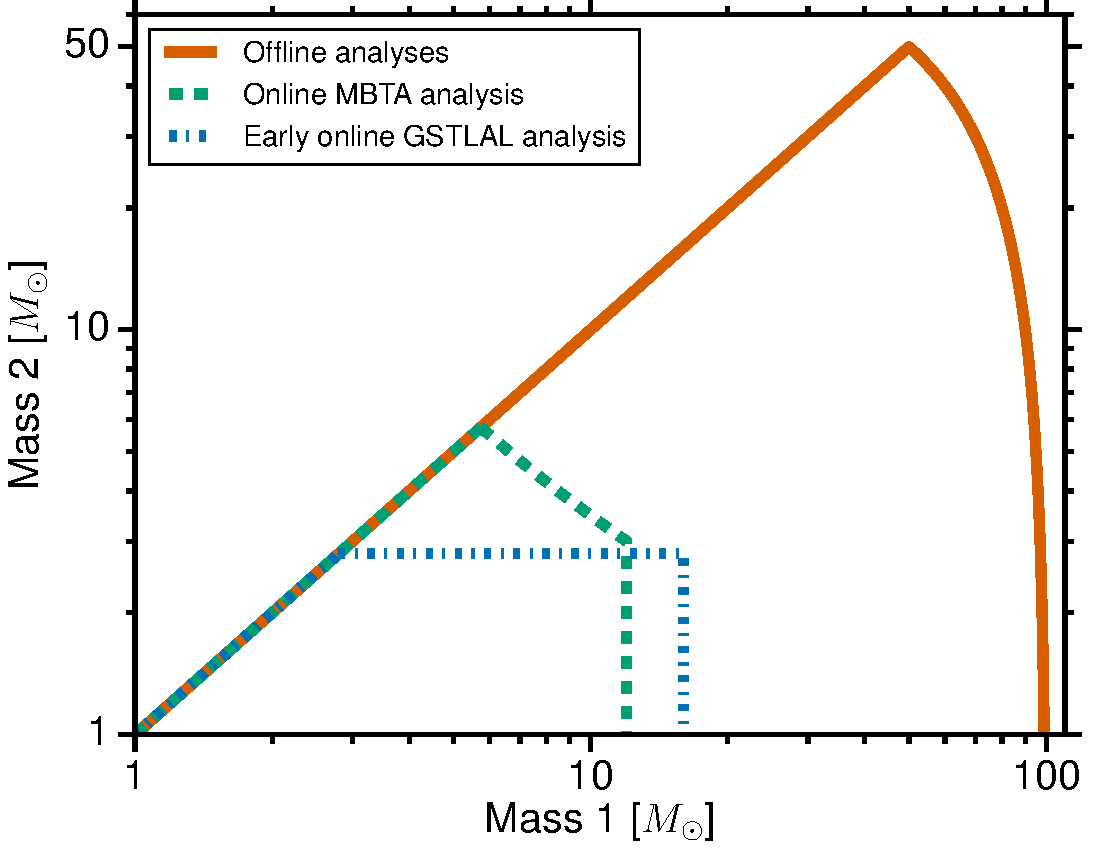
\includegraphics[width=\textwidth]{figs/chapter3/figure1}
\caption{\label{fig:banks}The range of template mass parameters considered for the
three different template banks used in the search.
The offline analyses, \pycbc\ and \gstlal\, used the largest
bank up to total masses of $100 M_{\odot}$. The online \gstlal\ analysis
used the larger bank after December 23, 2015.
The online \mbta\ bank covered primary masses below $12 M_{\odot}$
and chirp masses\textsuperscript{\ref{foot:note1}} below
$5 M_{\odot}$. The early online \gstlal\ bank up to December 23, 2015, covered primary
masses up to $16 M_{\odot}$ and secondary masses up to $2.8 M_{\odot}$.
The spin ranges are not shown here but are discussed in the text. }
\end{figure}

  \subsection{Offline Search}
  \label{ssec:offline_searches}
  The offline \ac{CBC} search of the \ac{O1} data set consists of two independently-implemented matched-filter
analyses: \gstlal~\citep{Messick:2016aqy} and
\pycbc~\citep{Usman:2015kfa}.
Full details of the \pycbc{}\ offline search pipeline are described in chapter~\ref{ch:GW150914_PyCBC_Offline}.

In contrast to the online search, the offline search uses data produced with
smaller calibration errors~\citep{Abbott:2016jsd}, uses complete information about the instrumental
data quality~\citep{TheLIGOScientific:2016zmo} and ensures that all available data is analysed.
The offline search in \ac{O1} forms a single search targeting \ac{BNS}, \ac{NSBH}, and \ac{BBH} systems. The
waveform filters cover systems with individual
component masses ranging from 1 to 99 $M_{\odot}$, total mass
constrained to less than 100 $M_{\odot}$ (see Figure~\ref{fig:banks}), and component dimensionless spins up to $\pm$ 0.05
for components with mass less than 2 $M_{\odot}$ and $\pm$ 0.99 otherwise~\citep{TheLIGOScientific:2016pea,Capano:2016dsf}.
Waveform filters with total mass less than 4 $M_{\odot}$ (chirp mass less than
$1.73 {M}_{\odot}$\footnote{\label{foot:note1}The
``chirp mass'' is the combination of the two component masses that
\ac{LIGO} is most sensitive to, given by $\mathcal{M} = (m_1 m_2)^{3/5} (m_1 + m_2)^{-1/5}$, where
$m_i$ denotes the two component masses})
for \pycbc\ (\gstlal) are modeled with the
inspiral-only, post-Newtonian, frequency-domain approximant
``TaylorF2''~\citep{Arun:2008kb,Bohe:2013cla,Blanchet:2013haa,Bohe:2015ana,mishra2016ready}.
At larger masses it becomes important to also include the merger and ringdown components of the waveform.
There a reduced-order model of the effective-one-body waveform calibrated against numerical
relativity is used~\citep{Taracchini:2013rva,Purrer:2015tud}. 


%  \subsection{Online Search}
%  \label{ssec:online_searches}
%  %The online \ac{CBC} search of the \ac{O1} data also consisted of two analyses;
%an online version of \gstlal\,\citep{Messick:2016aqy} and \mbta\,\citep{Adams:2015ulm}.
%For detailed descriptions of the \mbta\ analysis we refer the reader to~\citep{Beauville:2007kp,Virgo:2011aa,Adams:2015ulm}.
%The bank of waveform filters used by \gstlal\ up to December 23, 2015---and by
%\mbta\ for the duration of \ac{O1}---targeted systems that contained at least one \ac{NS}.
%Such systems are most likely to have an \ac{EM} counterpart, which would
%be powered by the material from a disrupted \ac{NS}.
%These sets of waveform filters were constructed using methods described
%in~\citep{Brown:2012qf,Harry:2013tca,Pannarale:2014rea}. \gstlal\ chose to cover systems with component masses of
%$m_1 \in [1,16] M_{\odot}; m_2 \in [1,2.8] M_{\odot}$ and \mbta\ covered $m_1, m_2 \in [1,12] M_{\odot}$ with
%a limit on chirp mass $\mathcal{M} < 5\mathrm{M}_{\odot}$ (see Figure~\ref{fig:banks}). In \gstlal\ component spins were
%limited to $\chi_{i} < 0.05$ for $m_{i} < 2.8\mathrm{M}_{\odot}$ and $\chi_{i} < 1$ otherwise, for
%\mbta\ $\chi_{i} < 0.05$ for $m_{i} < 2\mathrm{M}_{\odot}$ and $\chi_{i} < 1$ otherwise.
%\gstlal\ also chose to limit the template bank to include only systems for which it is possible for
%a \ac{NS} to have disrupted during the late inspiral using constraints described
%in~\citep{Pannarale:2014rea}. For the \mbta\ search the waveform filters were modelled using the
%``TaylorT4'' time-domain, post-Newtonian inspiral approximant~\citep{Buonanno:2009zt}.
%For \gstlal\
%the TaylorF2 frequency-domain, post-Newtonian waveform approximant was
%used~\citep{Arun:2008kb,Bohe:2013cla,Blanchet:2013haa,Bohe:2015ana,Mishra:2016whh}.
%All waveform models used in this paper are publicly available
%in the \texttt{lalsimulation} repository~\citep{LAL}.\footnote{The
%  internal \texttt{lalsimulation} names for the waveforms used as filters
%  described in this work are ``TaylorF2'' for the frequency-domain post-Newtonian
%  approximant, ``SpinTaylorT4'' for the time-domain
%  approximant used by \mbta\ and ``SEOBNRv2\_ROM\_DoubleSpin'' for the
%  aligned-spin effective one body waveform.
%  In addition, for calculation of rate estimates describe in Section \ref{sec:rates},
%  the ``SpinTaylorT4'' model is used to simulate BNS signals and
%  ``SEOBNRv3'' is used to simulate NSBH signals.}

%After December 23, 2015, and triggered by the discovery of GW150914, the \gstlal\
%analysis was extended to cover the same search space---using
%the same set of waveform filters---as the offline search~\citep{Capano:2016dsf,TheLIGOScientific:2016pea}.



  \subsection{Dataset}
  \label{ssec:dataset}
  Advanced \ac{LIGO}'s first observing run occurred between \OoneSTART\ and \OoneEND\
and consists of data from the two \ac{LIGO} observatories in Hanford, WA and Livingston, LA.
The LIGO detectors were running stably with roughly 40\% coincident operation, and had
been commissioned to roughly a third of the design sensitivity by the time of the start of O1~\citep{Martynov:2016fzi}.
During this observing run the final offline dataset consisted of \OoneOfflineAnalysableHTimeSeconds\
of analyzable data from the Hanford observatory, and \OoneOfflineAnalysableLTimeSeconds\ of data from the
Livingston observatory. We analyze only times during which \emph{both} observatories
took analyzable data, which is \OoneOfflineAnalysableTimeSeconds. Characterization studies of the analysable
data found \OoneOfflineAnalysableCatTwoDiffSeconds\ of coincident data during which time
there was some identified instrumental problem---known to
introduce excess noise---in at least one of the interferometers~\citep{TheLIGOScientific:2016zmo}.
These times are removed before assessing the significance of events
in the remaining analysis time. Some additional time is not analysed because
of restrictions on the minimal length of data segments and because of data lost
at the start and end of those segments~\citep{TheLIGOScientific:2016qqj, TheLIGOScientific:2016pea}.
These requirements are slightly different between the two offline analyses, \pycbc\ and \gstlal\. The \pycbc\
pipeline analysed 46.1 days of data.

\section{Search Results}
\label{sec:search_results}
%\begin{figure}[t]
%  \centering
%  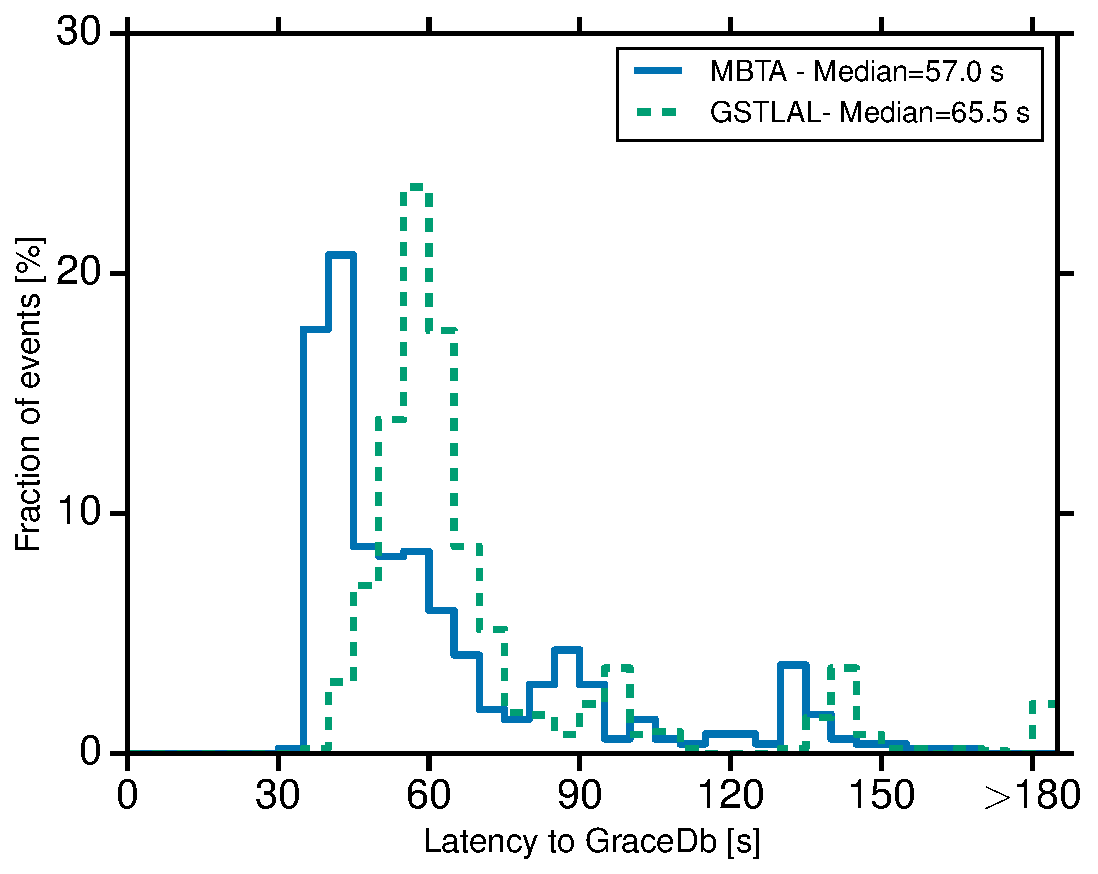
\includegraphics[width=1.0\textwidth]{figs/chapter3/figure2}
%  \caption{\label{fig:latency} Latency of the online searches during O1.
%           The latency is measured as the time between the event arriving at Earth
%           and time at which the event is uploaded to \ac{GraCEDb}.}
%\end{figure}

The offline search, targeting \ac{BBH} as well as \ac{BNS} and \ac{NSBH} mergers, identified
two signals with $> 5 \sigma$ confidence in the \ac{O1} dataset~\citep{Abbott:2016blz,Abbott:2016nmj}. A third signal was
also identified with \LVBLAHsignificance\ confidence~\citep{TheLIGOScientific:2016pea, TheLIGOScientific:2016qqj}. Subsequent
parameter inference on all three of these events has determined that, to very high
confidence, they were not produced by a \ac{BNS} or \ac{NSBH} merger~\citep{TheLIGOScientific:2016wfe, TheLIGOScientific:2016pea}. No other events
are significant with respect to the noise background in the offline search~\citep{TheLIGOScientific:2016pea}, and
we therefore state that no \ac{BNS} or \ac{NSBH} mergers were observed.

%The online search identified a total of \OoneOnlineTotalEMFollowUpEvents\ unique \ac{GW} candidate events
%with a false-alarm rate (FAR) less than
%$6\, \mathrm{yr}^{-1}$.
%Events with a FAR less than this are sent to electromagnetic partners if they
%pass event validation.
%Six of the events were rejected during the event validation as they were associated
%with known non-Gaussian behavior in one of the observatories. Of the remaining
%events, one was the \ac{BBH} merger GW151226 reported in~\citep{Abbott:2016nmj}. The second
%event identified by \gstlal\ was only narrowly below the FAR threshold, with a FAR of $3.1\, \mathrm{yr}^{-1}$.
%This event was also detected by \mbta\ with a higher FAR of $35\, \mathrm{yr}^{-1}$.
%This is consistent with noise in the online searches and the candidate event was later
%identified to have a false alarm rate of $190\, \mathrm{yr}^{-1}$
%in the offline \gstlal\ analysis.
%Nevertheless, the event passed all event validation and was released for \ac{EM} follow-up observations,
%which showed no significant counterpart. The results
%of the \ac{EM} follow-up program are discussed in more detail in~\citep{Abbott:2016gcq}.

%All events identified by the \gstlal\ or \mbta\ online analyses with a false alarm rate of less than
%$3200 \, \mathrm{yr}^{-1}$
%are uploaded to an internal database known
%as the \acf{GraCEDb}~\citep{gracedb}.
%In total \OoneOnlineTotalMBTAGraceDBEvents\ events were uploaded from \mbta\
%and \OoneOnlineTotalGSTLALGraceDBEvents\ from \gstlal.
%We can measure the latency of the online pipelines from the time between the
%inferred arrival time of each event at the Earth and the time at which the
%event is uploaded to \ac{GraCEDb}. This latency is illustrated in Fig.~\ref{fig:latency},
%where it can be seen that both online pipelines acheived median latencies on
%the order of one minute. We note that \gstlal\ uploaded twice as many events as \mbta\
%because of a difference in how the FAR was defined. The FAR reported by \mbta\ was defined
%relative to the rate of coincident data such that an event with a FAR of $1 \, \mathrm{yr}^{-1}$
%is expected to occur once in a year of coincident data. The FAR reported by \gstlal\ was defined 
%relative to wall-clock time such that an event with a FAR of $1 \, \mathrm{yr}^{-1}$
%is expected to occur once in a calendar year. In the following section we use the \mbta\
%definition of FAR when computing rate upper limits.


\section{Rates}
\label{sec:rates}
\subsection{Calculating upper limits}
\label{ssec:upper_limits}

Given no evidence for \ac{BNS} or \ac{NSBH} coalescences during \ac{O1}, we seek to place an upper limit
on the astrophysical rate of such events.
The expected number of observed events $\Lambda$ in a given analysis can be
related to the astrophysical rate of coalescences for a given source $R$ by
%
\begin{linenomath*}
\begin{equation}
\Lambda = R { \langle VT \rangle}.
\end{equation}
\end{linenomath*}
%
Here, $\langle VT \rangle$ is the space-time volume that the detectors are sensitive
to---averaged over space, observation time, and the parameters of the source population
of interest. The likelihood for finding zero observations in the data $s$ follows the
Poisson distribution for zero events $p(s | \Lambda) = e^{-\Lambda}$. Bayes' theorem then
gives the posterior for $\Lambda$
%
\begin{linenomath*}
\begin{equation}
p(\Lambda | s) \propto p(\Lambda) e^{-\Lambda},
\label{eq:lambdapost}
\end{equation}
\end{linenomath*}
%
where $p(\Lambda)$ is the prior on $\Lambda$.

Searches of Initial \ac{LIGO} and Initial Virgo data used a uniform prior on
$\Lambda$~\citep{Colaboration:2011np} but included prior information from previous searches. 
For the \ac{O1} \ac{BBH} search, however, a Jeffreys prior of
$p(\Lambda) \propto 1/\sqrt{\Lambda}$ for the Poisson likelihood was used~\citep{Farr:2013yna,Abbott:2016nhf,TheLIGOScientific:2016pea}.
A Jeffreys prior has the convenient property that the resulting posterior is invariant under a change in parametrization. 
However, for consistency with past BNS and NSBH results we will primarily use a uniform prior, and note that a Jeffreys
prior generally predicts a rate upper limit that is $\sim 40$\% smaller. 
We do not include additional prior information because the sensitive $\langle VT \rangle$ from 
all previous runs is an order of magnitude smaller than that of \ac{O1}.
We estimate $\langle VT \rangle$ by adding a large number of
simulated waveforms sampled from an astrophysical population into the data. 
These simulated signals
are recovered with an estimate of the FAR using the offline analyses.
Monte-Carlo integration methods are then utilized to estimate
the sensitive volume to which the detectors can recover gravitational-wave signals
below a chosen FAR threshold, which in this paper we will choose to be $0.01 \mathrm{yr}^{-1}$.
This threshold is low enough that only signals that are likely to be true events are counted as found, and we 
note that varying this threshold in the range 0.0001--1~yr$^{-1}$ only changes the calculated $\langle VT \rangle$ 
by about $\pm 20\%$.

Calibration uncertainties lead to a difference between the amplitude of simulated
waveforms and the amplitude of real waveforms with the same luminosity distance $d_L$.
During \ac{O1}, the $1\sigma$ uncertainty in the strain amplitude was 6\%, resulting
in an 18\% uncertainty in the measured $\langle VT \rangle$. Results presented here
also assume that injected waveforms are accurate
representations of astrophysical sources. We use a time-domain, aligned-spin,
post-Newtonian point-particle approximant to model \ac{BNS}
injections~\citep{Buonanno:2009zt}, and a time-domain, effective-one-body waveform
calibrated against numerical relativity to model \ac{NSBH}
injections~\citep{Pan:2013rra,Taracchini:2013rva}. Waveform differences between these models and
the offline search templates are therefore including in the calculated $\langle VT \rangle$. 
The injected NSBH waveform model is not calibrated at high mass ratios
($m_1/m_2 >8$), so there is some additional modeling uncertainty for large-mass NSBH
systems. The true sensitive volume $\langle VT \rangle$  will also be smaller if the effect of
tides in \ac{BNS} or \ac{NSBH} mergers is extreme. However, for most scenarios
the effects of waveform modeling will be smaller than the
effects of calibration errors and the choice of prior discussed above. 

The posterior on $\Lambda$ (Eq.~\ref{eq:lambdapost}) can be reexpressed as a joint
posterior on the astrophysical rate $R$ and the sensitive volume  $\langle VT \rangle$
\begin{linenomath*}
\begin{equation}
p(R, \langle VT \rangle | s) \propto p(R, \langle VT \rangle) e^{-R \langle VT \rangle}.
\end{equation}
\end{linenomath*}
%
The new prior can be expanded as $p(R, \langle VT \rangle) = p(R | \langle VT \rangle) p(\langle VT \rangle)$. 
For $p(R | \langle VT \rangle)$, we will either use a uniform prior on $R$ or a prior proportional to the 
Jeffreys prior $1/\sqrt{R \langle VT \rangle}$. As with Refs.~\citep{Abbott:2016nhf, Abbott:2016drs, TheLIGOScientific:2016pea}, 
we use a log-normal prior on $\langle VT \rangle$
%
\begin{linenomath*}
\begin{equation}
p(\langle VT \rangle) = \ln \mathcal{N}(\mu, \sigma^2),
\end{equation}
\end{linenomath*}
%
where $\mu$ is the calculated value of $\ln\langle VT \rangle$ and $\sigma$ represents the fractional uncertainty
in $\langle VT \rangle$. Below, we will use an uncertainty of
$\sigma=18\%$ due mainly to calibration errors.

Finally, a posterior for the rate is obtained by marginalizing over $\langle VT \rangle$
%
\begin{linenomath*}
\begin{equation}
p(R | s) = \int d\langle VT \rangle\, p(R, \langle VT \rangle | s).
\label{eq:posterior}
\end{equation}
\end{linenomath*}
%
The upper limit $R_c$ on the rate with confidence $c$ is then given by the solution to
%
\begin{linenomath*}
\begin{equation}
\label{eq:upperlimit}
\int_0^{R_c} dR\, p(R | s) = c.
\end{equation}
\end{linenomath*}

For reference, we note that in the limit of zero uncertainty in $\langle VT \rangle$,
the uniform prior for $p(R | \langle VT \rangle)$ gives a rate upper limit of
%
\begin{linenomath*}
\begin{equation}
R_c = \frac{ -\ln(1-c) }{ \langle VT \rangle },
\end{equation}
\end{linenomath*}
%
corresponding to $R_{90\%} = 2.303/\langle VT \rangle$ for a 90\% confidence upper
limit~\citep{Biswas:2007ni}. For a Jeffreys prior on $p(R | \langle VT \rangle)$, this upper limit is
%
\begin{linenomath*}
\begin{equation}
R_c = \frac{ [{\rm erf}^{-1}(c)]^2 }{ \langle VT \rangle },
\end{equation}
\end{linenomath*}
%
corresponding to $R_{90\%} = 1.353/\langle VT \rangle$ for a 90\% confidence upper limit.


\subsection{BNS rate limits}
\label{ssec:bns_rate_limits}

\begin{figure}[t]
   \centering
   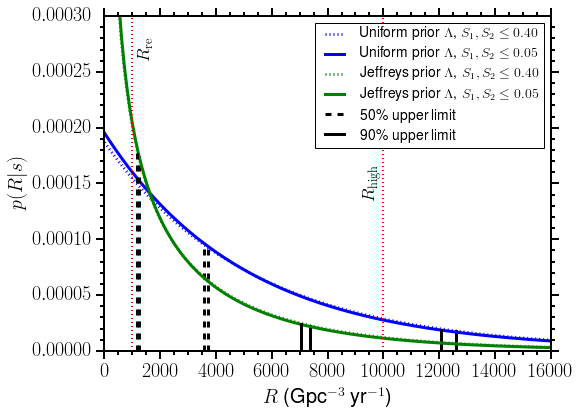
\includegraphics[width=\columnwidth]{figs/chapter3/figure3.png} 
   \caption{Posterior density on the rate of \ac{BNS} mergers calculated using the \pycbc\ analysis.
   Blue curves represent
   a uniform prior on the Poisson parameter $\Lambda = R \langle VT \rangle$, while
   green curves represent a Jeffreys prior on $\Lambda$. The solid (low spin population)
   and dotted (high spin population) posteriors almost overlap. The vertical dashed and
   solid lines represent the 50\% and 90\% confidence upper limits respectively for each
   choice of prior on $\Lambda$. For each pair of vertical lines, the left line is the 
   upper limit for the low spin population and the right line is the upper limit for the high
   spin population. Also shown are the realistic $R_{\rm re}$ and high end
   $R_{\rm high}$ of the expected \ac{BNS} merger rates identified in Ref.~\citep{Abadie:2010cf}.}
   \label{fig:bnspdf}
\end{figure}

\begin{figure}[t]
\centering
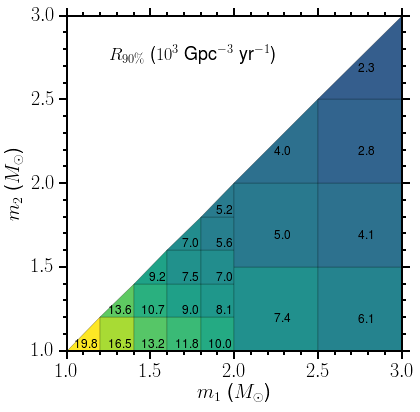
\includegraphics[width=1.0\textwidth]{figs/chapter3/figure4.png}
\caption{\label{fig:bns_ul_vs_mass} 90\% confidence upper limit on the \ac{BNS} merger rate as a function of the two component
masses using the \pycbc\ analysis. Here the upper limit for each bin is obtained assuming a \ac{BNS} population with masses distributed uniformly
within the limits of each bin, considering isotropic spin direction and dimensionless spin magnitudes uniformly
distributed in $[0, 0.05]$.}
\end{figure}

Motivated by considerations in Section \ref{sec:source_considerations}, we begin by
considering a population of \ac{BNS} sources with a narrow range of component
masses sampled from the normal distribution $\mathcal{N}(1.35M_\odot, (0.13M_\odot)^2)$
and truncated to remove samples outside the range $[1,3] M_{\odot}$. We consider
both a ``low spin'' \ac{BNS} population, where spins are distributed with uniform dimensionless
spin magnitude $\in [0, 0.05]$ and isotropic direction, and a ``high spin'' \ac{BNS}
population with a uniform dimensionless spin magnitude $\in [0, 0.4]$ and isotropic direction.
Our population uses an isotropic distribution of sky location and source orientation and chooses
distances assuming a uniform distribution in volume.
These simulations are modeled using a post-Newtonian waveform model, expanded using the
``TaylorT4'' formalism~\citep{Buonanno:2009zt}.
From this population we compute the space-time volume that Advanced \ac{LIGO} was
sensitive to during the O1 observing run. Results are shown for the measured $\langle VT\rangle$
in Table~\ref{tab:bns_ul_table} using a detection threshold of $\mathrm{FAR} = 0.01\, \mathrm{yr}^{-1}$.
Because the template bank for the searches use only aligned-spin \ac{BNS} templates with 
component spins up to 0.05, the \pycbc\ pipeline is 4\% more sensitive 
to the low-spin population than to the high-spin population.
The difference in $\langle VT\rangle$ between the two analyses is no larger than 5\%, which
is consistent with the difference in time analyzed in the two analyses. 
In addition, the calculated $\langle VT \rangle$
has a Monte Carlo integration uncertainty of $\sim1.5\%$ due to the finite number of injection
samples.

Using the measured $\langle VT \rangle$, the rate posterior and upper limit can be
calculated from Eqs.~\ref{eq:posterior} and~\ref{eq:upperlimit} respectively.
The posterior and upper limits are shown in Figure~\ref{fig:bnspdf} and depend
sensitively on the choice of uniform versus Jeffreys prior
for $\Lambda=R\langle VT \rangle$. However, they depend only weakly on the spin
distribution of the \ac{BNS} population and on the width $\sigma$ of the uncertainty
in $\langle VT \rangle$. For the conservative uniform prior on $\Lambda$ and an
uncertainty in $\langle VT \rangle$ due to calibration errors of 18\%, we find the
90\% confidence upper limit on the rate of \ac{BNS} mergers to be \MainBNSULLowSpin~Gpc$^{-3}$~yr$^{-1}$
for low spin and \MainBNSULHighSpin~Gpc$^{-3}$~yr$^{-1}$ for high spin using the values of $\langle VT \rangle$
calculated with \pycbc. These numbers can be compared to the upper limit 
computed from analysis of Initial \ac{LIGO} and Initial Virgo data~\citep{Colaboration:2011np}. 
There, the upper limit for $1.35$ -- $1.35 M_{\odot}$ non-spinning \ac{BNS} mergers is given 
as \SSixULNoSpin. The O1 upper limit is more than an order of magnitude lower than this previous upper limit.

To allow for uncertainties in the mass distribution of \ac{BNS} systems we also
derive 90\% confidence upper limits as a function of the \ac{NS} component masses.
To do this we construct a population of software injections with component masses
sampled uniformly in the range $[1, 3]M_{\odot}$, and an isotropic distribution
of component spins with magnitudes uniformly distributed in $[0, 0.05]$. We then bin
the \ac{BNS} injections by mass, and calculate $\langle VT \rangle$ and the associated 90\%
confidence rate upper limit for each bin. The 90\% rate upper limit for the conservative
uniform prior on $\Lambda$ as a function of component masses is shown in 
Figure~\ref{fig:bns_ul_vs_mass} for \pycbc. The fractional difference between the \pycbc\
and \gstlal\ results range from 1\% to 16\%.
%The upper limit for \gstlal\ is \red{$\sim x\%$} smaller.


\subsection{NSBH rate limits}
\label{ssec:nsbh_rate_limits}

\begin{figure}[t]
\centering
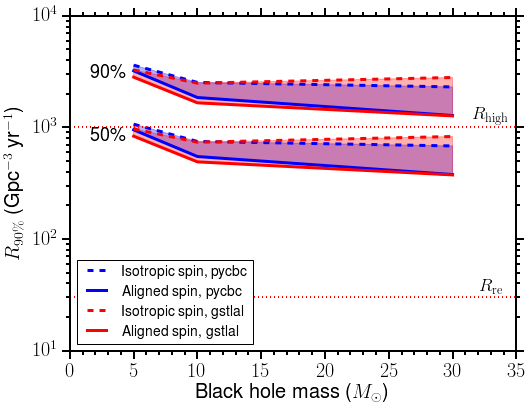
\includegraphics[width=1.0\textwidth]{figs/chapter3/figure5.png}
\caption{\label{fig:nsbh_ul_vs_mass} 50\% and 90\% upper limits on the \ac{NSBH} merger rate
as a function of the \ac{BH} mass using the more conservative uniform prior for the counts $\Lambda$. 
Blue curves represent the \pycbc\ analysis and red curves
represent the \gstlal\ analysis. The \ac{NS} mass is assumed to be $1.4M_\odot$. The spin magnitudes
were sampled uniformly in the range [0, 0.04] for \acp{NS} and [0, 1] for \acp{BH}. For the aligned
spin injection set, the spins of both the \ac{NS} and \ac{BH} are aligned (or anti-aligned) with the
orbital angular momentum. For the isotropic spin injection set, the orientation for the
spins of both the \ac{NS} and \ac{BH} are sampled isotropically. The isotropic spin distribution results
in a larger upper limit. Also shown are the realistic $R_{\rm re}$ and high end
$R_{\rm high}$ of the expected \ac{NSBH} merger rates identified in Ref.~\citep{Abadie:2010cf}.}
\end{figure}

Given the absence of known \ac{NSBH} systems and uncertainty in the \ac{BH} mass, we evaluate the
rate upper limit for a range of \ac{BH} masses. We use three masses that span the likely
range of \ac{BH} masses: $5M_\odot$, $10M_\odot$, and $30M_\odot$. For the \ac{NS} mass,
we use the canonical value of $1.4M_\odot$. We assume a distribution of \ac{BH} spin magnitudes
uniform in $[0,1]$ and \ac{NS} spin magnitudes uniform in $[0, 0.04]$.
For these three mass pairs, we compute upper limits for an isotropic spin distribution
on both bodies, and for a case where both spins are aligned or anti-aligned with the orbital angular momentum
(with equal probability of aligned vs anti-aligned).
Our NSBH population uses an isotropic distribution of sky location and source orientation and chooses
distances assuming a uniform distribution in volume. Waveforms are modeled
using the spin-precessing, effective-one-body model calibrated against numerical relativity
waveforms described in Ref.~\citep{Taracchini:2013rva,babak2016validating}.

The measured $\langle VT \rangle$ for a FAR threshold of $0.01 \mathrm{yr}^{-1}$ is given in Table~\ref{tab:nsbh_ul_table}
for \pycbc\. The uncertainty in the Monte Carlo integration of $\langle VT \rangle$ is 1.5\%--2\%. The corresponding 
90\% confidence upper limits are also given using the conservative 
uniform prior on $\Lambda$ and an 18\% uncertainty in $\langle VT
\rangle$. Analysis-specific differences in the limits range from 1\% to 20\%,
comparable or less than other uncertainties such as calibration.  
These results can be compared to the upper limits found for initial \ac{LIGO} and Virgo
for a population of $1.35M_\odot$--$5M_\odot$ \ac{NSBH} binaries with isotropic spin of
\SSixNSBHULFiveSpin at 90\% confidence~\citep{Colaboration:2011np}.
As with the \ac{BNS} case, this is an improvement in the upper limit of over an order of magnitude.

We also plot the 50\% and 90\% confidence upper limits from \pycbc\ and \gstlal\ as a function of mass in 
Figure~\ref{fig:nsbh_ul_vs_mass} for the uniform prior. The search is
less sensitive to isotropic spins than to (anti-)aligned spins due to two factors.
First, the volume-averaged signal
power is larger for a population of (anti-)aligned spin systems than for isotropic-spin systems.
Second, the search uses a template bank of (anti-)aligned spin systems, and thus loses sensitivity
when searching for systems with significantly misaligned spins.
As a result, the rate upper limits are less constraining
for the isotropic spin distribution than for the (anti-)aligned spin case.


\section{Astrophysical Interpretation}
\label{sec:astrophys_interp}

\begin{figure}[t]
\centering
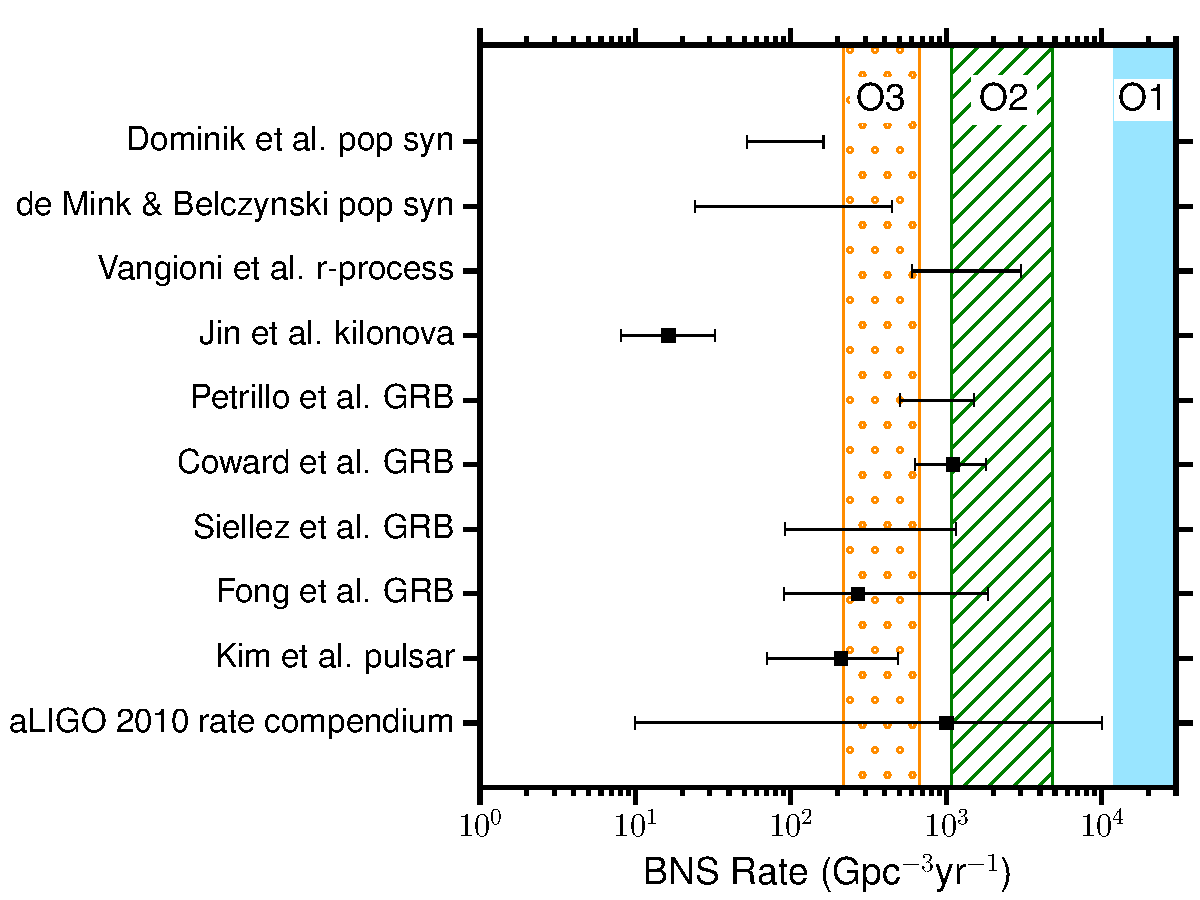
\includegraphics[width=\textwidth]{figs/chapter3/figure6}
\caption{\label{fig:ratecomparebns} A comparison of the \ac{O1} 90\% upper limit on the
\ac{BNS} merger rate to other rates discussed in the text \protect\citep{
Abadie:2010cf, Kim:2013tca, Fong:2015oha, Siellez:2013hia, Coward:2012gn,
Petrillo:2012ij, Jin:2015txa, Vangioni:2015ofa, deMink:2015yea, Dominik:2014yma}.  The region excluded by the low-spin \ac{BNS} rate limit is
shaded in blue.  Continued non-detection in O2 (slash) and O3 (dot) with higher
sensitivities and longer operation time would imply stronger upper limits.  The
O2 and O3 \ac{BNS} ranges are assumed to be 1-1.9 and 1.9-2.7 times larger than
\ac{O1}.  The operation times are assumed to be 6 and 9
months~\citep{Aasi:2013wya} with a duty cycle equal to that of \ac{O1} ($\sim$ 40\%).}
\end{figure}

\begin{figure}[t]
\centering
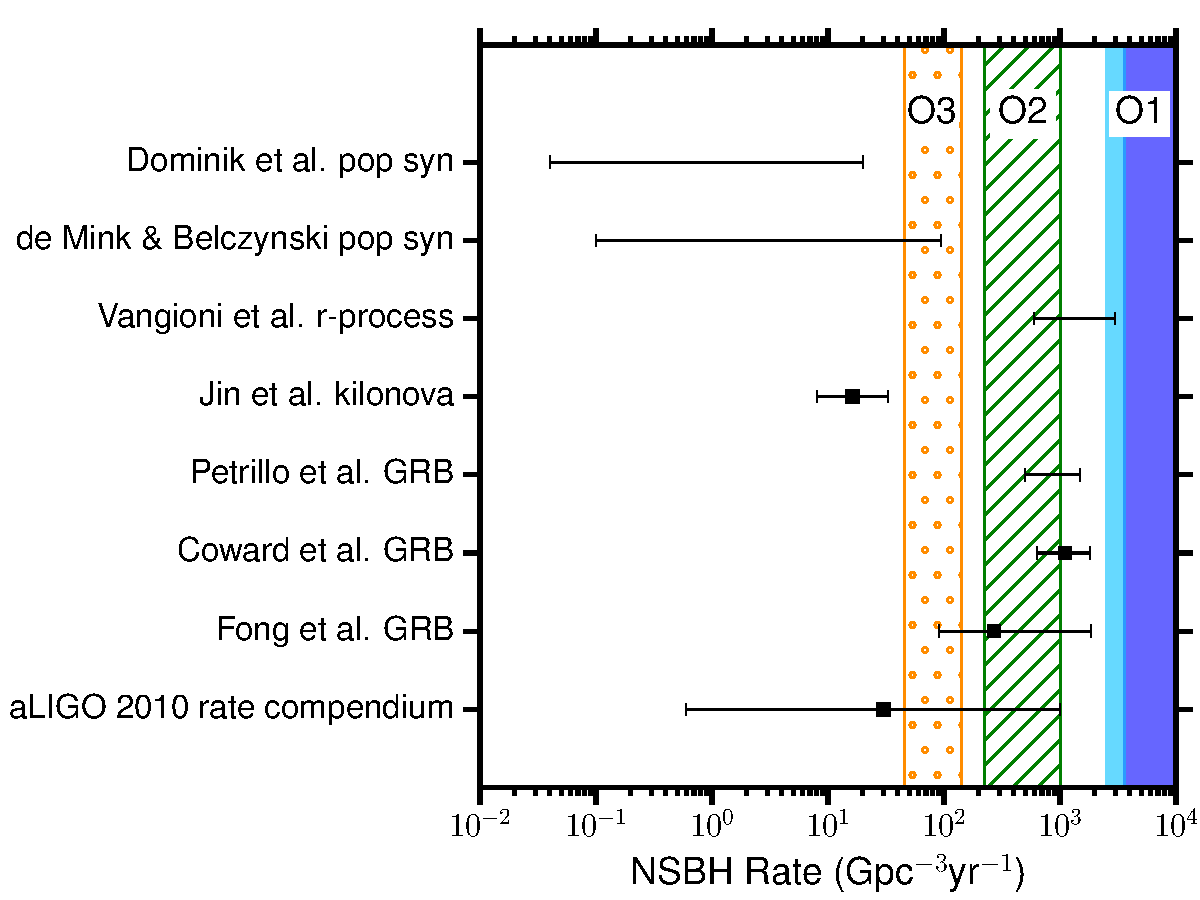
\includegraphics[width=\textwidth]{figs/chapter3/figure7}
\caption{\label{fig:ratecomparensbh} A comparison of the \ac{O1} 90\% upper limit on
the \ac{NSBH} merger rate to other rates discussed in
the text \protect\citep{Abadie:2010cf, Fong:2015oha, Coward:2012gn,
Petrillo:2012ij, Jin:2015txa, Vangioni:2015ofa, deMink:2015yea, Dominik:2014yma}.
The dark blue region assumes a \ac{NSBH} population with masses 5--1.4 $M_{\odot}$ and the
light blue region assumes a \ac{NSBH} population with masses 10--1.4 $M_{\odot}$.
Both assume an isotropic spin distribution.
Continued non-detection in O2 (slash) and O3 (dot) with higher sensitivities and longer
operation time would imply stronger upper limits (shown for 10--1.4 $M_{\odot}$ \ac{NSBH}
systems).
The O2 and O3 ranges are assumed to be 1-1.9 and 1.9-2.7 times larger than
\ac{O1}.
The operation times are assumed to be 6 and 9 months~\citep{Aasi:2013wya}
with a duty cycle equal to that of \ac{O1} ($\sim$ 40\%).}
\end{figure}

\begin{figure}[t]
\centering
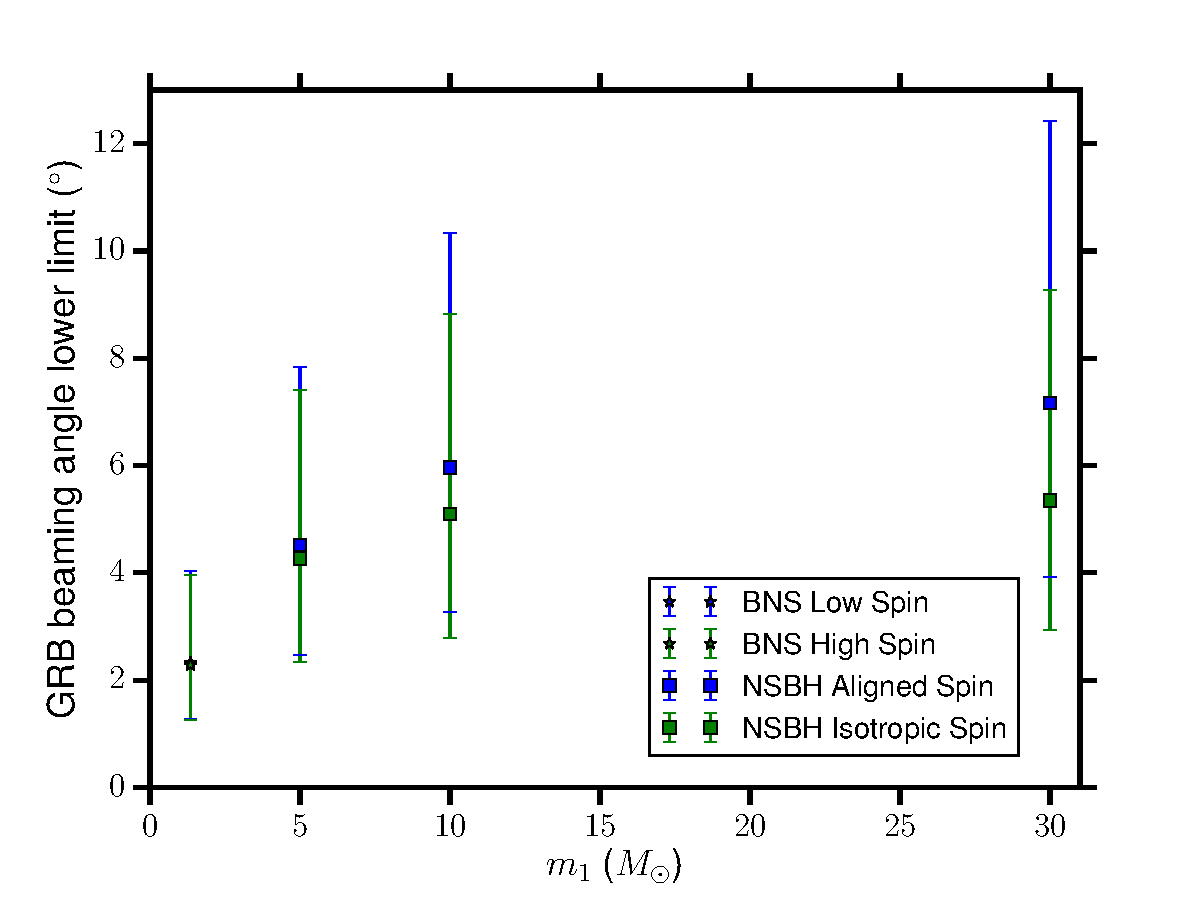
\includegraphics[width=\textwidth]{figs/chapter3/figure8.pdf}
\caption{\label{fig:beaming} Lower limit on the beaming angle of short
\acp{GRB}, as a function of the mass of the primary BH or
NS, $m_1$. We take the appropriate  90\% rate upper limit from this paper,
assume all short \acp{GRB} are produced by each case in turn, and assume all
have the same beaming angle $\theta_j$. The limit is calculated using an
observed short \ac{GRB} rate of
$10^{+20}_{-7}$Gpc$^{-3}$ yr$^{-1}$
and the ranges shown on the plot reflect the uncertainty in this observed rate.
For \ac{BNS}, $m_2$ comes from a Gaussian distribution centered on $1.35M_\odot$, and
for \ac{NSBH} it is fixed to $1.4M_\odot$.}
\end{figure}

We can compare our upper limits with rate predictions for compact object mergers
involving \acp{NS}, shown for \ac{BNS} in Figure~\ref{fig:ratecomparebns} and for \ac{NSBH} in
Figure~\ref{fig:ratecomparensbh}. A wide range of predictions derived from population
synthesis and from binary pulsar observations were reviewed in 2010 to produce rate estimates
for canonical
$1.4\,{{M_{\odot}}}$ \acp{NS} and $10\,{{M_{\odot}}}$ \acp{BH}~\citep{Abadie:2010cf}. We
additionally include some more recent estimates from population synthesis for
both \ac{NSBH} and \ac{BNS} \citep{Dominik:2014yma,Belczynski:2015tba,deMink:2015yea} and
binary pulsar observations for \ac{BNS} \citep{Kim:2013tca}.

We also compare our upper limits for \ac{NSBH} and \ac{BNS} systems to beaming-corrected
estimates of short \ac{GRB} rates in the local universe. Short \acp{GRB} are
considered likely to be produced by the merger of compact
binaries that include \acp{NS}, i.e. \ac{BNS} or \ac{NSBH}
systems~\citep{Berger:2013jza}. The rate of short \acp{GRB} can
predict the rate of progenitor mergers %\ac{BNS} and/or \ac{NSBH} systems
\citep{Coward:2012gn,Petrillo:2012ij,Siellez:2013hia,Fong:2015oha}.
For \ac{NSBH}, systems with small \ac{BH} masses are considered more likely to be able to
produce short \acp{GRB} (e.g.~ \citep{Duez:2009yz,Giacomazzo:2012zt,Pannarale:2015jia}), so we compare to our
$5 M_{\odot}$--$1.4 M_{\odot}$
\ac{NSBH} rate constraint. The observation of a kilonova is also considered to be an
indicator of a binary merger~\citep{Metzger:2011bv}, and an estimated kilonova rate
gives an additional lower bound on compact binary mergers~\citep{Jin:2015txa}.

Finally, some recent work has used the idea that mergers involving \acp{NS}
are the primary astrophysical source of r-process
elements \citep{1974ApJ...192L.145L,Qian:2007vq} to constrain the rate of such
mergers from nucleosynthesis \citep{Bauswein:2014vfa,Vangioni:2015ofa}, and we
include rates from \citep{Vangioni:2015ofa} for comparison.

While limits from \ac{O1} are not yet in tension with astrophysical models, scaling
our results to current expectations for advanced \ac{LIGO}'s next two observing runs,
O2 and O3 \citep{Aasi:2013wya}, suggests that significant constraints or
observations of \ac{BNS} or \ac{NSBH} mergers are possible in the next two years.

Assuming that short \acp{GRB} are produced by \ac{BNS} or \ac{NSBH}, but
without using beaming angle estimates, we can constrain the beaming angle of the jet
of gamma rays emitted from these \acp{GRB} by comparing the rates of
\ac{BNS}/\ac{NSBH} mergers and the rates of
short \acp{GRB}~\citep{Chen:2012qh}.
For simplicity, we assume here that all short \acp{GRB} are associated with \ac{BNS}
or \ac{NSBH} mergers; the true fraction will
depend on the emission mechanism.  The short \ac{GRB} rate $R_{GRB}$, the merger rate
$R_{merger}$, and the beaming angle $\theta_j$ are then related by
%
\begin{linenomath*}
\begin{equation}\label{eq:beaming}
\cos \theta_j = 1 - \frac{R_{\mathrm{GRB}}}{R_{\mathrm{merger}}}
\end{equation}
\end{linenomath*}

%
We take $R_{GRB}=10^{+20}_{-7}$Gpc$^{-3}$
yr$^{-1}$~\citep{Coward:2012gn,Nakar:2005bs}.
Figure~\ref{fig:beaming} shows the resulting \ac{GRB} beaming lower limits for the
90\% \ac{BNS} and \ac{NSBH} rate upper limits.
With our assumption that all short \ac{GRB}s are produced by a single progenitor
class, the constraint is tighter for \ac{NSBH} with larger
\ac{BH} mass.
Observed \ac{GRB} beaming angles are in the range of
$3-25^{\circ}$~\citep{Fox:2005kv,Fong:2015oha,Grupe:2006uc,Soderberg:2006bn,2013ApJ...766...41S,2012ApJ...756...63M,2011A&A...531L...6N}.
Compared to the lower limit derived from our non-detection, these \ac{GRB}
beaming observations start to confine the fraction of \ac{GRB}s that can be
produced by higher-mass NSBH as progenitor systems.
Future constraints could also come from \ac{GRB} and \ac{BNS} or \ac{NSBH} joint
detections~\citep{Dietz:2010eh,Regimbau:2014nxa, Clark:2014jpa}.

\section{Conclusion}
\label{sec:conclusion}

We report the non-detection of \ac{BNS} and \ac{NSBH} mergers in advanced \ac{LIGO}'s first observing run.
Given the sensitive volume of Advanced \ac{LIGO} to such systems we are able to place 90\%
confidence upper limits on the rates of \ac{BNS} and \ac{NSBH} mergers, improving upon limits
obtained from Initial \ac{LIGO} and Initial Virgo by roughly an order of magnitude.
Specifically we constrain the merger rate of \ac{BNS} systems with component masses of $1.35\pm0.13M_{\odot}$
to be less than \MainBNSULPyCBCHighSpin~Gpc$^{-3}$~yr$^{-1}$. We also constrain
the rate of \ac{NSBH} systems with NS masses of $1.4M_\odot$ and BH masses of at least $5M_{\odot}$ to be less than \MainNSBHULPyCBCFiveAligned~Gpc$^{-3}$~yr$^{-1}$ if
one considers a population where the component spins are (anti-)aligned with
the orbit, and less than \MainNSBHULPyCBCFiveIso~Gpc$^{-3}$~yr$^{-1}$ if one considers an isotropic distribution
of component spin directions.

We compare these upper limits with existing astrophysical rate models and find that the
current upper limits are in conflict with only the most optimistic models of the merger
rate. However, we expect that during the next two observing runs, O2 and O3, we will
either make observations of \ac{BNS} and \ac{NSBH} mergers or start placing significant constraints
on current astrophysical rates. Finally, we have explored the implications of this non-detection on
the beaming angle of short \acp{GRB}. We find that, if one assumes that all \acp{GRB}
are produced by \ac{BNS} mergers, then the opening angle of gamma-ray radiation must be larger
than \GRBBNSBeamingAngleConstraint; or larger than \GRBNSBHFiveBeamingAngleConstraint\ if
one assumes all \acp{GRB} are produced by \ac{NSBH} mergers.

